\section{Auswertung}
\label{sec:Auswertung}

\subsection{Bestimmung der spezifischen Elektronenladung}
Zur Erzeugung eines Magnetfeldes wurde eine Helmholtz-Spulenpaar verwendet mit den folgenden Abmessungen:
\begin{align*}
N &= 20 \\
R &= \SI{0,282}{\meter}
\end{align*}
wobei $N$ die Anzahl der Windungen und $R$ der Radius des Spulenpaares sind. In der Tabelle \ref{tab:Elladung} befinden sich die aufgeführten Stromstärken für die Ablenkung von oben auf den jeweils n-ten Strich. 

\begin{table}[htbp]
	\centering
	\caption{Messdaten für die Stromstärke $I$ und Abstand $\text{D}$ bei der Bestimmung der spezifischen Elektronenladung.}
	\label{tab:Elladung}
	\begin{tabular}{c c c c c c c}
		\toprule
		& $U_{\text{B}} / \si{\volt} $ & $250$ & $300$ & $350$ & $400$ & $440$ \\
		\midrule
		n & $\text{D} / \si{\m}$ & $I / \si{\ampere} $ & $I / \si{\ampere} $ & $I / \si{\ampere} $ & $I / \si{\ampere} $ & $I / \si{\ampere} $ \\
		\midrule
		1 &	0 &	0 & 0 & 0 &	0 & 0 \\
		2 &	0,006 &	0,3 &	0,3 &	0,4	 & 0,35 &	0,39 \\
		3 &	0,012 &	0,625&	0,625 &	0,8	 & 0,7  &	0,82 \\
		4 &	0,019 &	0,95 &	0,99 &	1,15 & 1,14 &	1,24 \\
		5 &	0,025 &	1,25 &	1,325&	1,5	 & 1,5	&   1,63 \\
		6 &	0,031 &	1,55 &	1,65 &	1,9	 & 1,9	&   2,04 \\
		7 &	0,038 &	1,85 &	1,98 &	2,3	 & 2,3	&   2,95 \\
		8 &	0,044 &	2,5  &  2,36 &  2,69 & 2,73	&   2,95 \\
		9 &	0,050 & -    &  2,725 &	3,95 & 3,15 &	3,26 \\
		\bottomrule
	\end{tabular}
\end{table}

Eine lineare Ausgleichsgerade lässt sich berechnen wie:
\begin{equation}
\label{eq:ausgleichsgerade}
y = mx + b
\end{equation}
wobei $m$ die Steigung und $b$ der y-Achsenabschnitt sind. Mit der Gleichung \ref{eq:ausgleichsgerade} werden die Steigungen und die Fehler der Ausgleichsgeraden vom Python-Modul Scipy curve\_fit berechnet.
Zuerst wird mithilfe der Gleichung \ref{eqn:magfeld} die magnetische Feldstärke berechnet. Danach wird die Größe $\frac{D}{(L^2+D^2)}$ mit den Werten für $D$ aus der Tabelle \ref{tab:Elladung} ermittelt, wobei $L = \SI{0,175}{\meter}$ beträgt. Die errechneten Werte befinden sich nun in der Tabelle \ref{tab:Neu} und diese werden in die Abildungen \ref{fig:v250}, \ref{fig:v300}, \ref{fig:v350}, \ref{fig:v400} und \ref{fig:v440} eingetragen.

\begin{table}[htbp]
	\centering
	\caption{Die neuen errechneten Ergebnisse mit Hilfe der Messwerte für die Bestimmung der spezifischen Elektronenladung.}
	\label{tab:Neu}
	\begin{tabular}{c c c c c c}
		\toprule
		$\frac{D}{(L^2+D^2)}$ & $B / \si{\micro\tesla}$ & $B / \si{\micro\tesla}$ & $B / \si{\micro\tesla}$ & $B / \si{\micro\tesla}$ & $B / \si{\micro\tesla}$ \\
		\midrule
		0	  & 0     &	0       &	0	& 0	& 0 \\
		0,207 &	19,13 &	19,13	& 25,50 &	22,32	& 24,87 \\
		0,412 &	39,85 &	39,85	& 51,01 &	44,64	& 52,29 \\
		0,614 &	60,58 &	63,13	& 73,33 &	72,69	& 79,07 \\
		0,812 &	79,71 &	84,49	& 95,65 &	95,65	& 103,94 \\
		1,003 &	98,84 &	105,22	& 121,16 &	121,16  &	130,09 \\
		1,187 &	117,97  & 126,26&	146,67 &	146,67 &	188,12 \\
		1,363 &	159,42	& 150,50&	171,54 &	174,09 &	188,12 \\
		1,529 &	- &	173,77 & 251,89&	200,87 &	207,89 \\
		\bottomrule
	\end{tabular}
\end{table}

Die Steigungen betragen dann wie folgt:
\begin{align*}
m_{250} &= \SI{8619,32 \pm 596,00}{\frac{1}{\tesla\meter}} \\
m_{300} &= \SI{8619,11 \pm 181,48}{\frac{1}{\tesla\meter}} \\
m_{350} &= \SI{6166,17 \pm 665,03}{\frac{1}{\tesla\meter}} \\
m_{400} &= \SI{7393,47 \pm 177,70}{\frac{1}{\tesla\meter}} \\
m_{440} &= \SI{6729,39 \pm 409,05}{\frac{1}{\tesla\meter}}.
\end{align*}
Die y-Achsenabschnitte betragen auch die folgenden Werte:
\begin{align*}
b_{250} &= \SI{0,091 \pm 0,055}{\tesla} \\
b_{300} &= \SI{0,070 \pm 0,019}{\tesla} \\
b_{350} &= \SI{0,169 \pm 0,090}{\tesla} \\
b_{400} &= \SI{0,079 \pm 0,021}{\tesla} \\
b_{440} &= \SI{0,071 \pm 0,056}{\tesla}.
\end{align*}

\begin{figure}[h!]
	\centering
	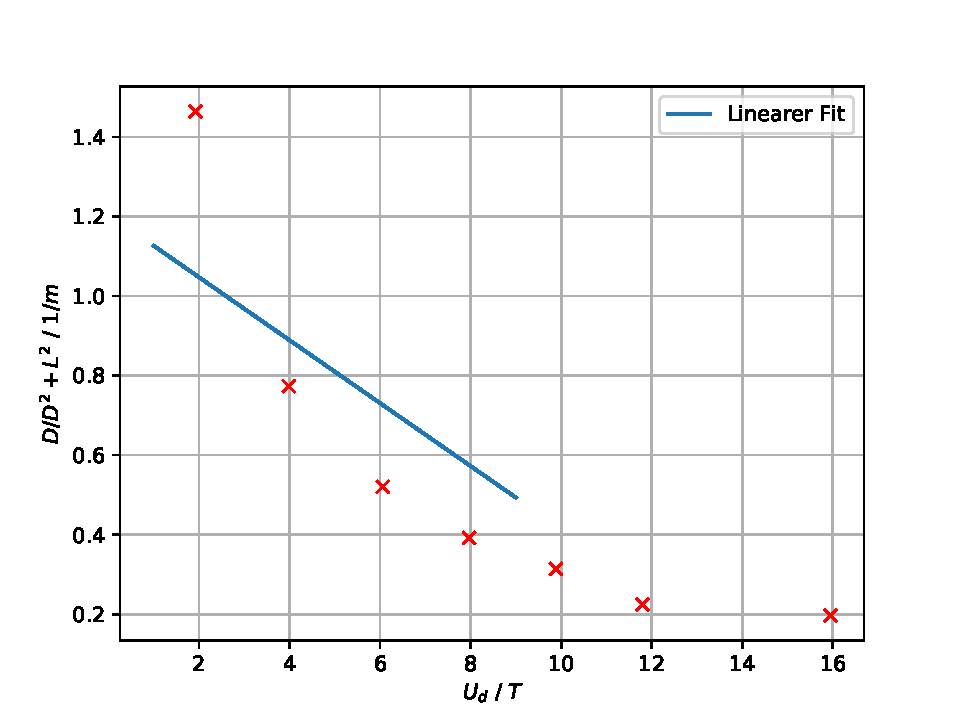
\includegraphics[width=0.7\linewidth]{../../V250}
	\caption{Die Messwerte und zugehörige Ausgleichsgerade für die Beschleunigungsspannung $U_\text{B} = \SI{250}{\volt}$.}
	\label{fig:v250}
\end{figure}

\begin{figure}[h!]
	\centering
	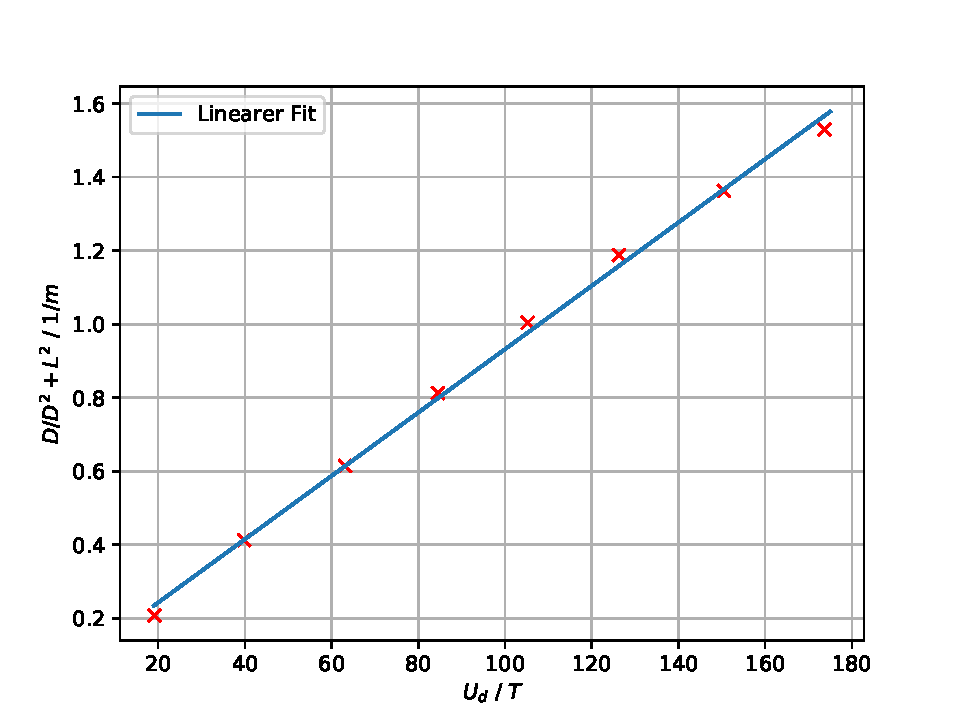
\includegraphics[width=0.7\linewidth]{../../V300}
	\caption{Die Messwerte und zugehörige Ausgleichsgerade für die Beschleunigungsspannung $U_\text{B} = \SI{300}{\volt}$.}
	\label{fig:v300}
\end{figure}

\begin{figure}[h!]
	\centering
	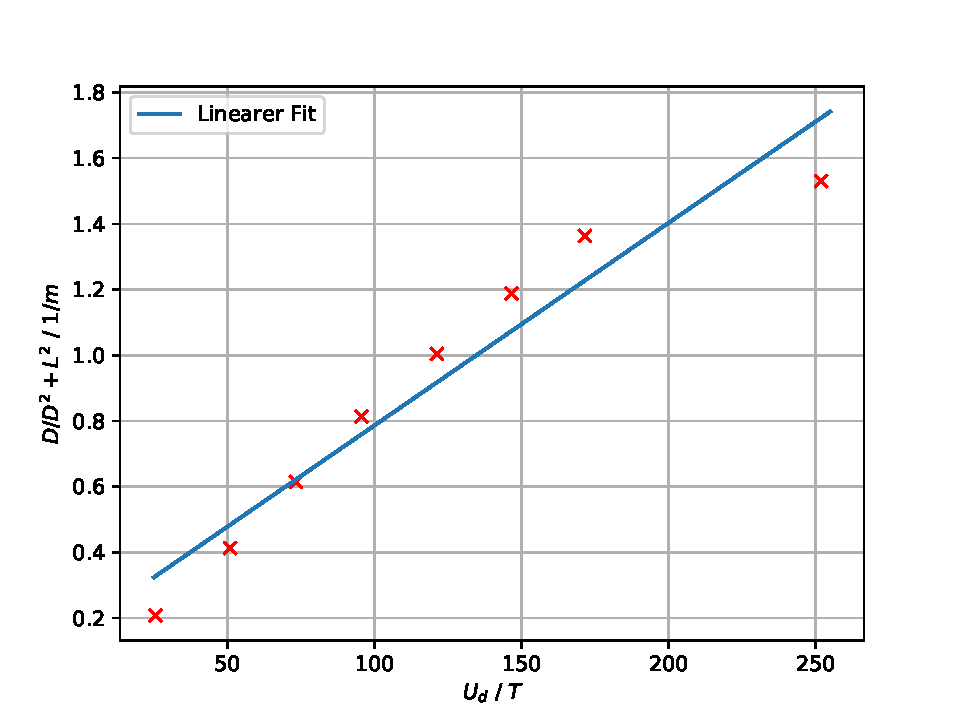
\includegraphics[width=0.7\linewidth]{../../V350}
	\caption{Die Messwerte und zugehörige Ausgleichsgerade für die Beschleunigungsspannung $U_\text{B} = \SI{350}{\volt}$.}
	\label{fig:v350}
\end{figure}

\begin{figure}[h!]
	\centering
	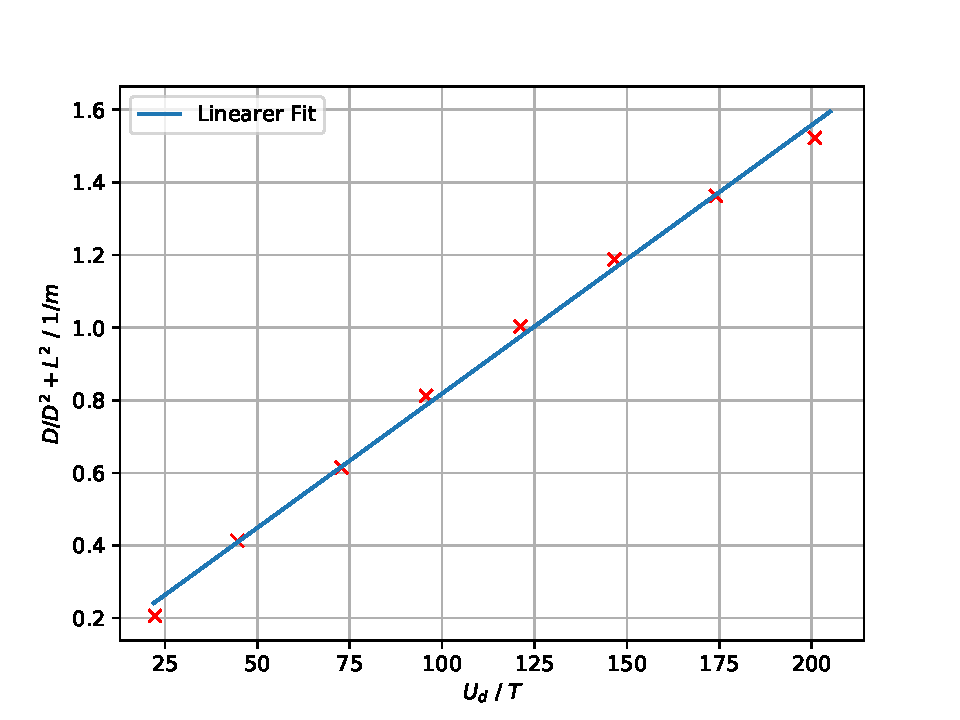
\includegraphics[width=0.7\linewidth]{../../V400}
	\caption{Die Messwerte und zugehörige Ausgleichsgerade für die Beschleunigungsspannung $U_\text{B} = \SI{400}{\volt}$.}
	\label{fig:v400}
\end{figure}

\begin{figure}[h!]
	\centering
	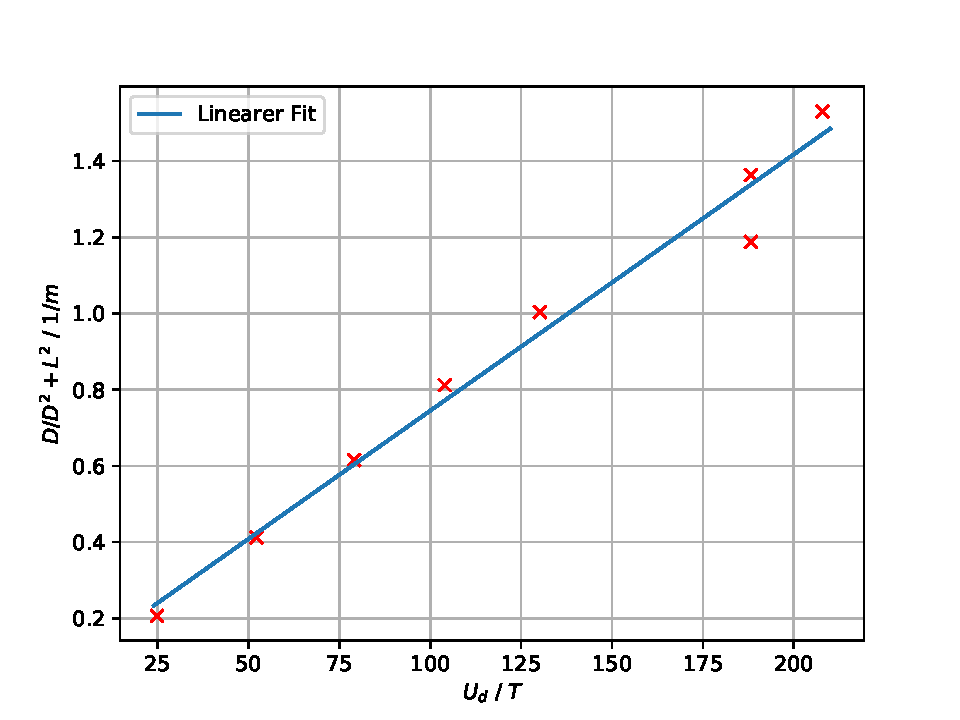
\includegraphics[width=0.7\linewidth]{../../V440}
	\caption{Die Messwerte und zugehörige Ausgleichsgerade für die Beschleunigungsspannung $U_\text{B} = \SI{440}{\volt}$.}
	\label{fig:v440}
\end{figure}

Es ist darauf zu achten, dass bei der Steigung und y-Achsenabschnitt als Index die jeweilige Beschleunigungsspannung steht. Für die Berechnung der spezifischen Elektronenladung wird die Gleichung \ref{eqn:letzte} benutzt und entsprechend nach der gesuchten Größe umgeschrieben:
\begin{equation}
\label{eq:spezladung}
 \frac{e_0}{m_0} =  \left[\frac{D}{L^2+D^2}\left(\frac{\sqrt{8U_\text{B}}}{B}\right)\right]^2.
\end{equation}
und vereinfacht sich mit der eben berechneten Steigungen zu:
\begin{equation}
\label{eq:spezladung2}
\frac{e_0}{m_0} = 8U_\text{B} a^2.
\end{equation}

Danach wird in die Gleichung \ref{eq:spezladung2} die Steigungen sowie die benutzten Beschleunigungsspannungen eingesetzt und es ergeben sich die folgenden spezifischen Ladungen:
\begin{align*}
\frac{e_0}{m_0} &= \SI{1,485 \pm 0,007}{\coulomb\per\kg} \text{für 250V} \\
\frac{e_0}{m_0} &= \SI{1,779 \pm 0,008}{\coulomb\per\kg} \text{für 300V} \\
\frac{e_0}{m_0} &= \SI{1,064 \pm 0,012}{\coulomb\per\kg} \text{für 350V} \\
\frac{e_0}{m_0} &= \SI{1,749 \pm 0,001}{\coulomb\per\kg} \text{für 400V} \\
\frac{e_0}{m_0} &= \SI{1,594 \pm 0,005}{\coulomb\per\kg} \text{für 440V}.
\end{align*}

Die Formel für den Mittelwert $\bar{x}$ aus $n$ Stichproben $x_{i}$ ergibt sich aus:
\begin{equation}
\bar{x}=\frac{1}{n}\sum \limits_{i=1}^n x_{i}.
\label{eq:mittelwert}
\end{equation}
Mit der Gleichung \ref{eq:mittelwert} wird der Mittelwert für die spezifische Elektronenladung berechnet und es ergibt sich:
\begin{equation}
\label{eq:mittelwertspez}
\frac{e_0}{m_0} = \SI{1,534 \pm 0,006}{\coulomb\per\kg}.
\end{equation}

\subsection{Bestimmung des lokalen Erdmagnetfeldes}
Der mittels eines Deklinatorium-Inklinatoriums bestimmte Inklinationswinkel ergibt sich zu $70,1$ Grad. 

Aus dem Spulenstrom lässt sich das durch die Spule erzeugte Magnetfeld $B_{\text{tot}}$ bestimmen. Um daraus $B_{\text{hor}}$ zu bestimmen, also das Feld, dass das Erdmagnetfeld kompensiert, wird $B_{\text{tot}}$ durch den Cosinus des zuvor bestimmten Winkels geteilt. 

Durch die Gleichung \ref{eqn:magfeld} mit einem Spulenstrom von $I=\SI{0,26}{\ampere}$ ergibt sich $B_{\text{tot}}=\SI{16,5}{\micro\tesla}$ und folglich:
\begin{align*}
B_{\text{hor}} = \frac{B_{\text{tot}}}{\text{cos}(70,1)}=\SI{48,4}{\micro\tesla}.
\end{align*}

